\documentclass{article}
\usepackage{xeCJK}
\usepackage{amsmath}
\usepackage{graphicx}

\setCJKmainfont{Microsoft YaHei}
\linespread{1.5}
\setlength{\parindent}{0pt}


\begin{document}
一.\\
\begin{figure}[htbp]
    \centering
    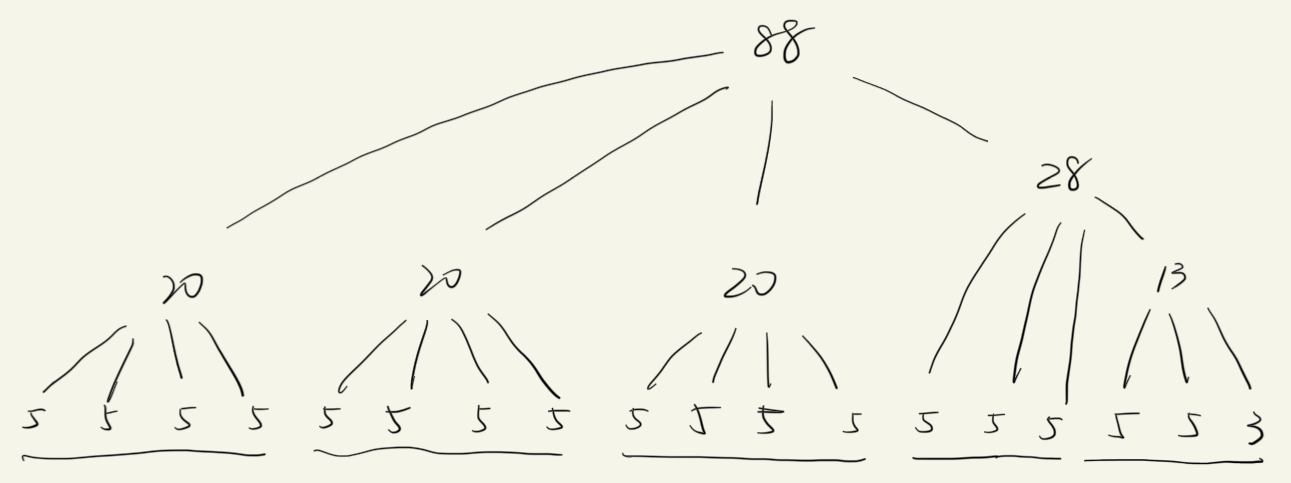
\includegraphics[scale=0.4]{tree.png}
    \caption{归并树}
\end{figure}
磁盘总读写次数:
$88 \times 2 + (20 + 20 + 20 + 13) \times 2 + 28 \times 2 + 88 \times 2 = 554$
\\
二. \\
选中 $A = 10$ 的概率: 
\[\frac{1}{20},\]
选中 $B = 20$ 的概率: 
\[\frac{1}{10},\]
选中 $A = 10\; \text{and}\; B = 20$ 的概率: 
\[\frac{1}{20} \times \frac{1}{10} = \frac{1}{200},\]
故选中 $A = 10\; \text{or}\; B = 20$ 的概率: 
\[\frac{1}{20} + \frac{1}{10} - \frac{1}{200} = \frac{29}{200},\]
大小为: 
\[10000 \times \frac{29}{200} = 1450.\]
\end{document}